% Options for packages loaded elsewhere
\PassOptionsToPackage{unicode}{hyperref}
\PassOptionsToPackage{hyphens}{url}
%
\documentclass[
  12pt,
]{article}
\usepackage{amsmath,amssymb}
\usepackage{iftex}
\ifPDFTeX
  \usepackage[T1]{fontenc}
  \usepackage[utf8]{inputenc}
  \usepackage{textcomp} % provide euro and other symbols
\else % if luatex or xetex
  \usepackage{unicode-math} % this also loads fontspec
  \defaultfontfeatures{Scale=MatchLowercase}
  \defaultfontfeatures[\rmfamily]{Ligatures=TeX,Scale=1}
\fi
\usepackage{lmodern}
\ifPDFTeX\else
  % xetex/luatex font selection
\fi
% Use upquote if available, for straight quotes in verbatim environments
\IfFileExists{upquote.sty}{\usepackage{upquote}}{}
\IfFileExists{microtype.sty}{% use microtype if available
  \usepackage[]{microtype}
  \UseMicrotypeSet[protrusion]{basicmath} % disable protrusion for tt fonts
}{}
\makeatletter
\@ifundefined{KOMAClassName}{% if non-KOMA class
  \IfFileExists{parskip.sty}{%
    \usepackage{parskip}
  }{% else
    \setlength{\parindent}{0pt}
    \setlength{\parskip}{6pt plus 2pt minus 1pt}}
}{% if KOMA class
  \KOMAoptions{parskip=half}}
\makeatother
\usepackage{xcolor}
\usepackage[margin=1in]{geometry}
\usepackage{color}
\usepackage{fancyvrb}
\newcommand{\VerbBar}{|}
\newcommand{\VERB}{\Verb[commandchars=\\\{\}]}
\DefineVerbatimEnvironment{Highlighting}{Verbatim}{commandchars=\\\{\}}
% Add ',fontsize=\small' for more characters per line
\usepackage{framed}
\definecolor{shadecolor}{RGB}{248,248,248}
\newenvironment{Shaded}{\begin{snugshade}}{\end{snugshade}}
\newcommand{\AlertTok}[1]{\textcolor[rgb]{0.94,0.16,0.16}{#1}}
\newcommand{\AnnotationTok}[1]{\textcolor[rgb]{0.56,0.35,0.01}{\textbf{\textit{#1}}}}
\newcommand{\AttributeTok}[1]{\textcolor[rgb]{0.13,0.29,0.53}{#1}}
\newcommand{\BaseNTok}[1]{\textcolor[rgb]{0.00,0.00,0.81}{#1}}
\newcommand{\BuiltInTok}[1]{#1}
\newcommand{\CharTok}[1]{\textcolor[rgb]{0.31,0.60,0.02}{#1}}
\newcommand{\CommentTok}[1]{\textcolor[rgb]{0.56,0.35,0.01}{\textit{#1}}}
\newcommand{\CommentVarTok}[1]{\textcolor[rgb]{0.56,0.35,0.01}{\textbf{\textit{#1}}}}
\newcommand{\ConstantTok}[1]{\textcolor[rgb]{0.56,0.35,0.01}{#1}}
\newcommand{\ControlFlowTok}[1]{\textcolor[rgb]{0.13,0.29,0.53}{\textbf{#1}}}
\newcommand{\DataTypeTok}[1]{\textcolor[rgb]{0.13,0.29,0.53}{#1}}
\newcommand{\DecValTok}[1]{\textcolor[rgb]{0.00,0.00,0.81}{#1}}
\newcommand{\DocumentationTok}[1]{\textcolor[rgb]{0.56,0.35,0.01}{\textbf{\textit{#1}}}}
\newcommand{\ErrorTok}[1]{\textcolor[rgb]{0.64,0.00,0.00}{\textbf{#1}}}
\newcommand{\ExtensionTok}[1]{#1}
\newcommand{\FloatTok}[1]{\textcolor[rgb]{0.00,0.00,0.81}{#1}}
\newcommand{\FunctionTok}[1]{\textcolor[rgb]{0.13,0.29,0.53}{\textbf{#1}}}
\newcommand{\ImportTok}[1]{#1}
\newcommand{\InformationTok}[1]{\textcolor[rgb]{0.56,0.35,0.01}{\textbf{\textit{#1}}}}
\newcommand{\KeywordTok}[1]{\textcolor[rgb]{0.13,0.29,0.53}{\textbf{#1}}}
\newcommand{\NormalTok}[1]{#1}
\newcommand{\OperatorTok}[1]{\textcolor[rgb]{0.81,0.36,0.00}{\textbf{#1}}}
\newcommand{\OtherTok}[1]{\textcolor[rgb]{0.56,0.35,0.01}{#1}}
\newcommand{\PreprocessorTok}[1]{\textcolor[rgb]{0.56,0.35,0.01}{\textit{#1}}}
\newcommand{\RegionMarkerTok}[1]{#1}
\newcommand{\SpecialCharTok}[1]{\textcolor[rgb]{0.81,0.36,0.00}{\textbf{#1}}}
\newcommand{\SpecialStringTok}[1]{\textcolor[rgb]{0.31,0.60,0.02}{#1}}
\newcommand{\StringTok}[1]{\textcolor[rgb]{0.31,0.60,0.02}{#1}}
\newcommand{\VariableTok}[1]{\textcolor[rgb]{0.00,0.00,0.00}{#1}}
\newcommand{\VerbatimStringTok}[1]{\textcolor[rgb]{0.31,0.60,0.02}{#1}}
\newcommand{\WarningTok}[1]{\textcolor[rgb]{0.56,0.35,0.01}{\textbf{\textit{#1}}}}
\usepackage{graphicx}
\makeatletter
\def\maxwidth{\ifdim\Gin@nat@width>\linewidth\linewidth\else\Gin@nat@width\fi}
\def\maxheight{\ifdim\Gin@nat@height>\textheight\textheight\else\Gin@nat@height\fi}
\makeatother
% Scale images if necessary, so that they will not overflow the page
% margins by default, and it is still possible to overwrite the defaults
% using explicit options in \includegraphics[width, height, ...]{}
\setkeys{Gin}{width=\maxwidth,height=\maxheight,keepaspectratio}
% Set default figure placement to htbp
\makeatletter
\def\fps@figure{htbp}
\makeatother
\setlength{\emergencystretch}{3em} % prevent overfull lines
\providecommand{\tightlist}{%
  \setlength{\itemsep}{0pt}\setlength{\parskip}{0pt}}
\setcounter{secnumdepth}{-\maxdimen} % remove section numbering
\usepackage{graphicx}
\usepackage{fancyhdr}
\usepackage{mdframed}
\pagestyle{fancy}
\fancyhead{}
\fancyhead[L]{\includegraphics[width=3cm]{logo.jpg}}
\fancyhead[R]{\hspace{0.5cm} Universidad Diego Portales \\ Facultad de Administración y Economía}
\fancypagestyle{plain}{ \fancyhead{} \fancyhead[L]{\includegraphics[width=3cm]{logo.jpg}} \fancyhead[R]{\hspace{0.5 cm} Universidad Diego Portales \\ Facultad de Administración y Economía}}
\usepackage{booktabs}
\usepackage{longtable}
\usepackage{array}
\usepackage{multirow}
\usepackage{wrapfig}
\usepackage{float}
\usepackage{colortbl}
\usepackage{pdflscape}
\usepackage{tabu}
\usepackage{threeparttable}
\usepackage{threeparttablex}
\usepackage[normalem]{ulem}
\usepackage{makecell}
\usepackage{xcolor}
\ifLuaTeX
  \usepackage{selnolig}  % disable illegal ligatures
\fi
\usepackage{bookmark}
\IfFileExists{xurl.sty}{\usepackage{xurl}}{} % add URL line breaks if available
\urlstyle{same}
\hypersetup{
  pdftitle={Ejercicio 4},
  hidelinks,
  pdfcreator={LaTeX via pandoc}}

\title{\textbf{Ejercicio 4}}
\author{}
\date{\vspace{-2.5em}}

\begin{document}
\maketitle

\maketitle
\vspace{-5em}
\vspace{0.5em}

\begin{center}
\footnotesize \textbf{Curso}: Econometría II \\
\footnotesize \textbf{Profesor}: Mauricio Tejada \\
\footnotesize \textbf{Estudiantes}: Dania Bustamante, Rosana Cardona, José Casanova \\
\footnotesize 5 junio 2024 \\
\end{center}

\section{Pregunta 1}\label{pregunta-1}

\emph{Creación de variables}

\begin{Shaded}
\begin{Highlighting}[]
\NormalTok{base }\OtherTok{\textless{}{-}}\NormalTok{ base }\SpecialCharTok{\%\textgreater{}\%}
  \FunctionTok{mutate}\NormalTok{(}\AttributeTok{log\_PIB =} \FunctionTok{log}\NormalTok{(PIB), }\AttributeTok{log\_fbcf =} \FunctionTok{log}\NormalTok{(fbcf)) }\SpecialCharTok{\%\textgreater{}\%}
  \FunctionTok{mutate}\NormalTok{(}\AttributeTok{d\_log\_PIB =}\NormalTok{ log\_PIB }\SpecialCharTok{{-}} \FunctionTok{lag}\NormalTok{(log\_PIB), }
         \AttributeTok{d\_log\_fbcf =}\NormalTok{ log\_fbcf }\SpecialCharTok{{-}} \FunctionTok{lag}\NormalTok{(log\_fbcf))}\SpecialCharTok{\%\textgreater{}\%}\FunctionTok{na.omit}\NormalTok{()}

\FunctionTok{head}\NormalTok{(base, }\DecValTok{4}\NormalTok{)}
\end{Highlighting}
\end{Shaded}

\begin{verbatim}
## # A tibble: 4 x 7
##   Periodo     fbcf    PIB log_PIB log_fbcf d_log_PIB d_log_fbcf
##   <date>     <dbl>  <dbl>   <dbl>    <dbl>     <dbl>      <dbl>
## 1 1961-01-01 2702. 20199.    9.91     7.90    0.0537     0.0128
## 2 1962-01-01 3033. 20993.    9.95     8.02    0.0386     0.116 
## 3 1963-01-01 3481. 22187.   10.0      8.16    0.0553     0.138 
## 4 1964-01-01 3283. 22733.   10.0      8.10    0.0243    -0.0587
\end{verbatim}

\begin{Shaded}
\begin{Highlighting}[]
\CommentTok{\# Convertir a series de tiempo}
\NormalTok{log\_PIB\_ts }\OtherTok{\textless{}{-}} \FunctionTok{ts}\NormalTok{(base}\SpecialCharTok{$}\NormalTok{log\_PIB, }\AttributeTok{start =} \FunctionTok{c}\NormalTok{(}\DecValTok{1960}\NormalTok{, }\DecValTok{1}\NormalTok{), }\AttributeTok{frequency =} \DecValTok{12}\NormalTok{)}
\NormalTok{log\_fbcf\_ts }\OtherTok{\textless{}{-}} \FunctionTok{ts}\NormalTok{(base}\SpecialCharTok{$}\NormalTok{log\_fbcf, }\AttributeTok{start =} \FunctionTok{c}\NormalTok{(}\DecValTok{1960}\NormalTok{, }\DecValTok{1}\NormalTok{), }\AttributeTok{frequency =} \DecValTok{12}\NormalTok{)}
\NormalTok{d\_log\_PIB\_ts }\OtherTok{\textless{}{-}} \FunctionTok{ts}\NormalTok{(base}\SpecialCharTok{$}\NormalTok{d\_log\_PIB, }\AttributeTok{start =} \FunctionTok{c}\NormalTok{(}\DecValTok{1960}\NormalTok{, }\DecValTok{1}\NormalTok{), }\AttributeTok{frequency =} \DecValTok{12}\NormalTok{)}
\NormalTok{d\_log\_fbcf\_ts }\OtherTok{\textless{}{-}} \FunctionTok{ts}\NormalTok{(base}\SpecialCharTok{$}\NormalTok{d\_log\_fbcf, }\AttributeTok{start =} \FunctionTok{c}\NormalTok{(}\DecValTok{1960}\NormalTok{, }\DecValTok{1}\NormalTok{),}\AttributeTok{frequency=}\DecValTok{12}\NormalTok{)}
\end{Highlighting}
\end{Shaded}

\subsection{\texorpdfstring{\emph{Gráficos series de
tiempo}}{Gráficos series de tiempo}}\label{gruxe1ficos-series-de-tiempo}

\begin{center}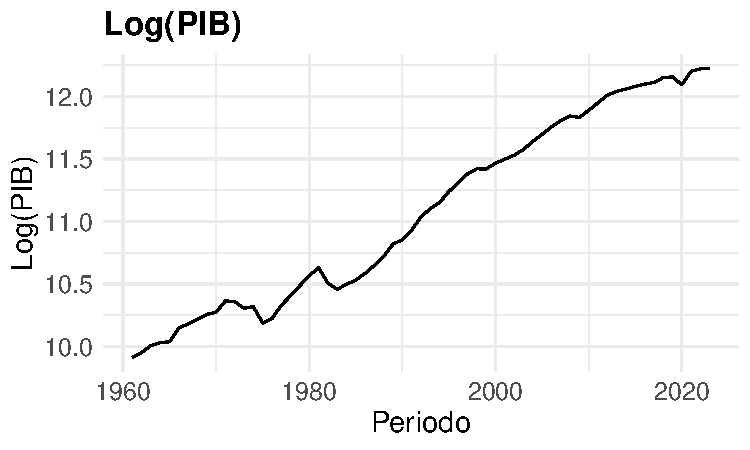
\includegraphics{ensayo_files/figure-latex/unnamed-chunk-5-1} \end{center}

\begin{center}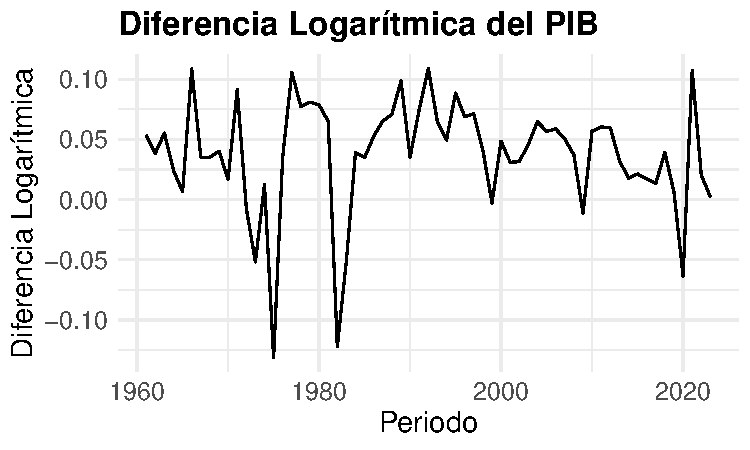
\includegraphics{ensayo_files/figure-latex/unnamed-chunk-6-1} \end{center}

\begin{center}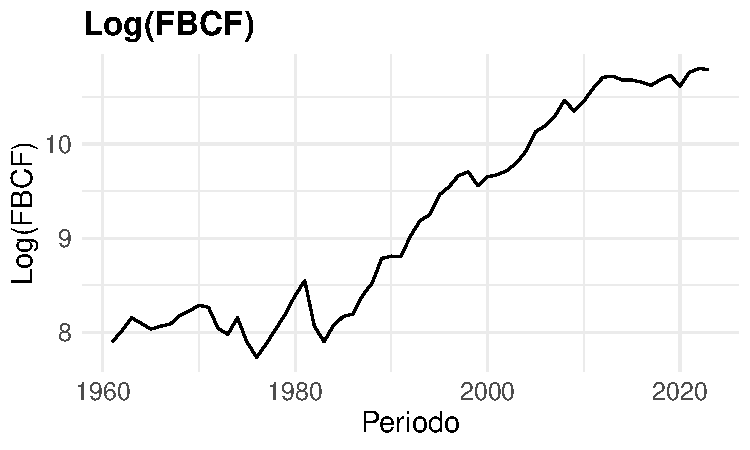
\includegraphics{ensayo_files/figure-latex/unnamed-chunk-7-1} \end{center}

\begin{center}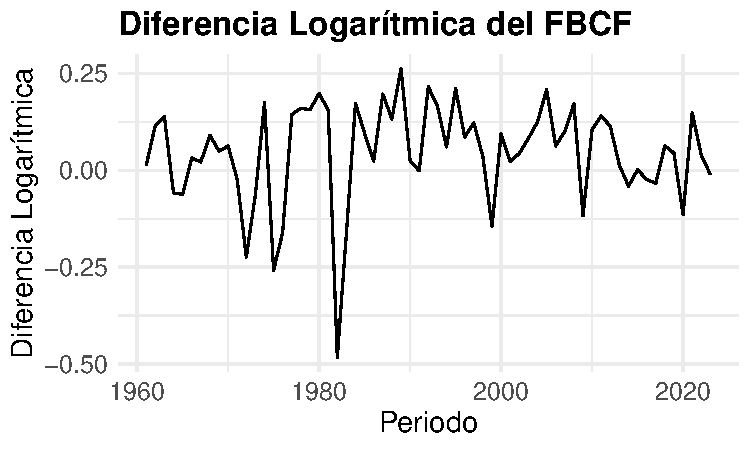
\includegraphics{ensayo_files/figure-latex/unnamed-chunk-8-1} \end{center}

\begin{itemize}
\item
  El gráfico muestra la evolución del logaritmo del PIB a lo largo del
  tiempo. Se observa una tendencia ascendente a lo largo del período
  analizado, indicando un crecimiento continuo del PIB en términos
  logarítmicos.
\item
  Diferencia Logarítmica del PIB: El gráfico de las diferencias
  logarítmicas del PIB muestra fluctuaciones alrededor de cero. Esto
  indica que, si bien el PIB tiene una tendencia ascendente, sus cambios
  logarítmicos son estacionarios alrededor de un valor medio.
\item
  Log(FBCF): Similar al PIB, el gráfico del logaritmo de la FBCF muestra
  una tendencia ascendente a lo largo del tiempo. Esto indica un
  crecimiento continuo de la FBCF en términos logarítmicos.
\item
  Diferencia Logarítmica del FBCF: El gráfico de las diferencias
  logarítmicas de la FBCF muestra fluctuaciones alrededor de cero. Esto
  indica que, aunque la FBCF tiene una tendencia ascendente, sus cambios
  logarítmicos son estacionarios alrededor de un valor medio.
\end{itemize}

\subsubsection{\texorpdfstring{\emph{Funciones de
autocorrelación}}{Funciones de autocorrelación}}\label{funciones-de-autocorrelaciuxf3n}

\begin{center}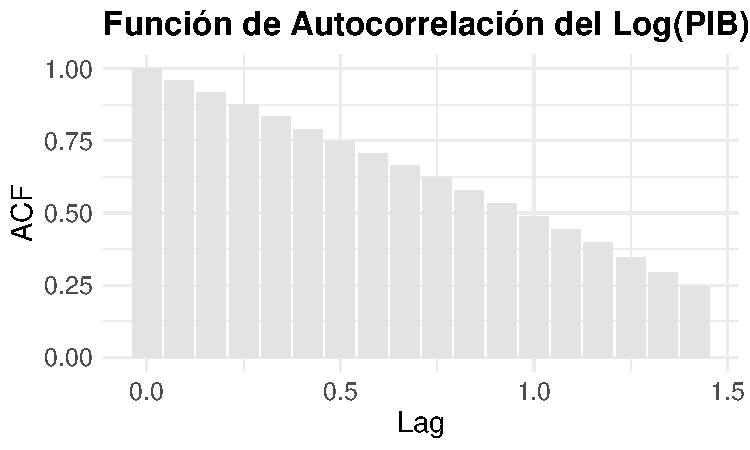
\includegraphics{ensayo_files/figure-latex/unnamed-chunk-12-1} \end{center}

\begin{center}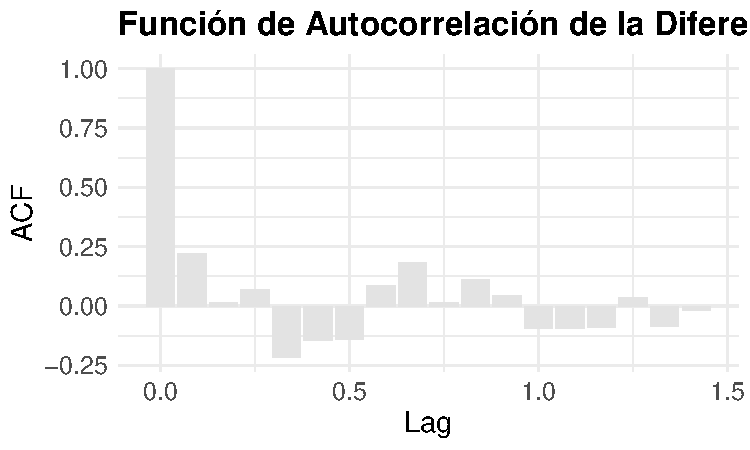
\includegraphics{ensayo_files/figure-latex/unnamed-chunk-13-1} \end{center}

\begin{center}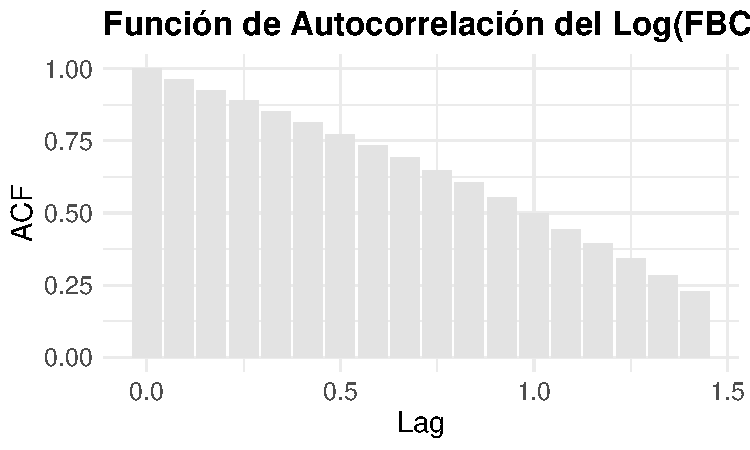
\includegraphics{ensayo_files/figure-latex/unnamed-chunk-14-1} \end{center}

\begin{center}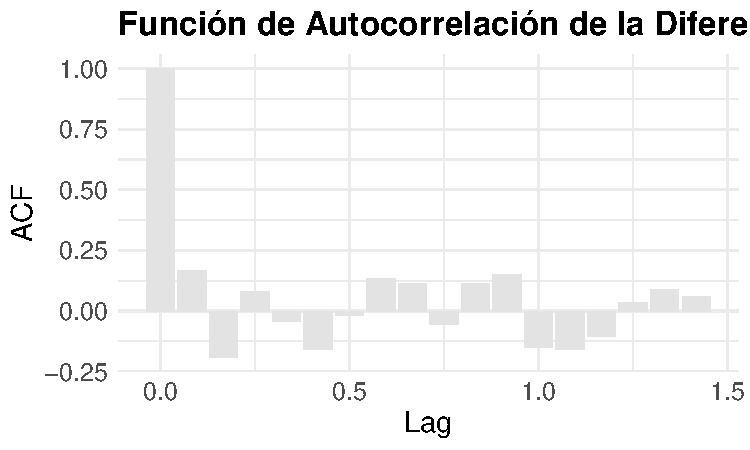
\includegraphics{ensayo_files/figure-latex/unnamed-chunk-15-1} \end{center}

\begin{itemize}
\item
  \emph{Función de Autocorrelación del Log(PIB):} Las autocorrelaciones
  decrecen lentamente, lo que indica una alta persistencia en la serie
  log(PBI). Esto sugiere que los valores pasados del log(PIB) tienen una
  fuerte influencia en los valores futuros.
\item
  \emph{Función de Autocorrelación de la Diferencia Logarítmica del
  PIB:} Las autocorrelaciones caen rápidamente a valores cercanos a cero
  después de los primeros rezagos. Esto indica que la serie de
  diferencias logarítmicas del PIB es estacionaria, con poca o ninguna
  persistencia.
\item
  \emph{Función de Autocorrelación del Log(FBCF):} Similar al log(PIB),
  las autocorrelaciones del log(FBCF) decrecen lentamente. Esto indica
  una alta persistencia en la serie log(FBCF), sugiriendo que los
  valores pasados tienen una fuerte influencia en los valores futuros.
\item
  F\emph{unción de Autocorrelación de la Diferencia Logarítmica del
  FBCF}: Las autocorrelaciones de las diferencias logarítmicas del FBCF
  también caen rápidamente a valores cercanos a cero. Esto indica que la
  serie de diferencias logarítmicas de la FBCF es estacionaria, con poca
  o ninguna persistencia.
\end{itemize}

Tanto el log(PIB) como el log(FBCF) muestran alta persistencia, lo que
indica que los valores pasados tienen una fuerte influencia en los
valores futuros.

\emph{Estacionariedad en las Diferencias Logarítmicas:} Las series de
diferencias logarítmicas del PIB y de la FBCF son estacionarias, lo que
indica que los cambios logarítmicos no muestran persistencia y fluctúan
alrededor de un valor medio constante. Estas observaciones sugieren que,
mientras que las series logarítmicas muestran tendencias a largo plazo,
sus diferencias logarítmicas se comportan de manera más aleatoria y
estacionaria. Esto es consistente con la teoría de que las series de
nivel (logarítmicas) pueden ser no estacionarias, pero sus diferencias
logarítmicas tienden a ser estacionarias.

\section{Pregunta 2}\label{pregunta-2}

\begin{verbatim}
##   Model   AIC_PIB  AIC_fbcf
## 1 AR(1) -200.2737 -72.86098
## 2 AR(2) -194.0268 -72.16490
## 3 AR(3) -188.2456 -69.98135
## 4 AR(4) -187.2141 -67.90005
\end{verbatim}

\begin{itemize}
\item
  \emph{Para Difflog(PIB):} el modelo que minimiza el AIC es AR(1).
\item
  \emph{Para Difflog(FBCF):} el modelo que minimiza el AIC es AR(1).
\item
  \emph{Difflog(PIB):} El modelo AR(1) tiene el menor AIC (-195.9572),
  indicando que es el modelo más adecuado para capturar la dinámica de
  las diferencias logarítmicas del PIB. Esto sugiere que un solo rezago
  del Difflog(PIB) es suficiente para modelar la serie de tiempo de
  manera eficiente.
\item
  \emph{Difflog(FBCF):} El modelo AR(1) también tiene el menor AIC
  (-70.94062), indicando que es el modelo más adecuado para capturar la
  dinámica de las diferencias logarítmicas de la FBCF. Similar a
  Difflog(PIB), un solo rezago del Difflog(FBCF) es suficiente para
  modelar la serie de tiempo de manera eficiente.
\end{itemize}

Para ambas series temporales (Difflog(PIB) y Difflog(FBCF)), el modelo
AR(1) es el que minimiza el AIC, indicando que este es el modelo más
eficiente para capturar las características de estas series. Este
resultado sugiere que las diferencias logarítmicas del PIB y de la FBCF
son bien modeladas considerando solo el primer rezago.

\section{Pregunta 3}\label{pregunta-3}

\begin{verbatim}
## Analysis of Variance Table
## 
## Response: d_log_PIB_ts
##                    Df   Sum Sq   Mean Sq F value  Pr(>F)  
## L(d_log_PIB_ts, 1)  1 0.006871 0.0068706  3.1632 0.08038 .
## Residuals          60 0.130323 0.0021721                  
## ---
## Signif. codes:  0 '***' 0.001 '**' 0.01 '*' 0.05 '.' 0.1 ' ' 1
\end{verbatim}

\begin{verbatim}
## Analysis of Variance Table
## 
## Response: d_log_fbcf_ts
##                     Df  Sum Sq  Mean Sq F value Pr(>F)
## L(d_log_fbcf_ts, 1)  1 0.02973 0.029732  1.7533 0.1905
## Residuals           60 1.01746 0.016958
\end{verbatim}

Resultados del Test F:

\begin{itemize}
\tightlist
\item
  Difflog(PIB)
\item
  Estadístico F: 3.1121
\item
  Valor p: 0.08289
\end{itemize}

El valor p es 0.08289, que es mayor que 0.05 pero menor que 0.1. Esto
indica que hay evidencia marginal (al nivel de significancia del 10\%)
para rechazar la hipótesis nula de que el coeficiente del rezago de
Difflog(PIB) es igual a cero.

En otras palabras, aunque no es significativo al 5\%, hay una indicación
de que el rezago de Difflog(PIB) puede tener un impacto en la serie de
tiempo, aunque esta evidencia no es fuerte.

La significancia marginal al nivel del 10\% sugiere que el rezago de
Difflog(PIB) podría tener un efecto en la serie, aunque esta evidencia
no es fuerte.

\begin{itemize}
\tightlist
\item
  Difflog(FBCF)
\item
  Estadístico F: 1.7834
\item
  Valor p: 0.1869
\end{itemize}

El valor p es 0.1869, que es mayor que 0.05 y también mayor que 0.1.
Esto indica que no hay suficiente evidencia para rechazar la hipótesis
nula de que el coeficiente del rezago de Difflog(FBCF) es igual a cero.
En otras palabras, el rezago de Difflog(FBCF) no parece ser
significativamente diferente de cero, sugiriendo que no tiene un impacto
considerable en la serie de tiempo.

No hay suficiente evidencia para concluir que el rezago de Difflog(FBCF)
tiene un efecto significativo en la serie.

En resumen, los resultados indican que el modelo AR(1) para Difflog(PIB)
podría ser marginalmente significativo, mientras que el modelo AR(1)
para Difflog(FBCF) no muestra evidencia de significancia. Esto sugiere
que debemos tener cautela al interpretar la importancia del rezago de
Difflog(PIB) y que probablemente se necesitan más datos o modelos más
complejos para capturar la dinámica de Difflog(FBCF).

\section{Pregunta 4}\label{pregunta-4}

\begin{verbatim}
##    Año Predicción_d_log_PIB Predicción_d_log_FBCF
## 1 2024           0.02920957            0.03676731
## 2 2025           0.03527941            0.04485000
## 3 2026           0.03664274            0.04621336
\end{verbatim}

\emph{Para Difflog(PIB):} En 2024, se espera que el crecimiento
logarítmico del PIB sea de aproximadamente 2.92\%. En 2025, el
crecimiento logarítmico del PIB se incrementa a aproximadamente 3.53\%.
En 2026, el crecimiento logarítmico del PIB se estabiliza ligeramente en
3.67\%. Estas predicciones indican un crecimiento continuo en el PIB,
con una tendencia positiva a lo largo de los tres años, lo cual sugiere
una recuperación o expansión económica sostenida.

\emph{Para Difflog(FBCF):} En 2024, se espera que el crecimiento
logarítmico de la FBCF sea de aproximadamente 3.54\%. En 2025, el
crecimiento logarítmico de la FBCF aumenta a aproximadamente 4.34\%. En
2026, el crecimiento logarítmico de la FBCF se estabiliza ligeramente en
4.47\%. Estas predicciones indican un incremento constante en la FBCF,
sugiriendo un aumento en la inversión en capital fijo, lo cual es una
señal positiva para la economía ya que puede conducir a un aumento en la
capacidad productiva y la eficiencia.

Las predicciones de Difflog(PIB) y Difflog(FBCF) para los años 2024,
2025 y 2026 muestran una tendencia de crecimiento continuo tanto en el
PIB como en la FBCF. Esto sugiere que la economía se está expandiendo,
con aumentos constantes en la producción y la inversión en capital fijo.

\section{Pregunta 5}\label{pregunta-5}

\begin{verbatim}
##               Año  log_PIB log_FBCF      PIB     FBCF
##              2023 12.22465 10.78888 203750.0 48478.74
## last_log_PIB 2024 12.25386 10.82565 209789.2 50294.35
## log_PIB_2024 2025 12.28914 10.87050 217322.6 52601.40
## log_PIB_2025 2026 12.32578 10.91671 225433.6 55089.33
\end{verbatim}

\begin{itemize}
\item
  Se observa un crecimiento continuo en el PIB a lo largo de los años,
  lo que sugiere una expansión económica sostenida.
\item
  Similar al PIB, la FBCF muestra un crecimiento continuo a lo largo de
  los años, indicando un aumento en la inversión en capital fijo.
\end{itemize}

Los valores calculados para el PIB muestran un crecimiento constante
desde 203750.0 en 2023 hasta 225459.0 en 2026, lo que indica una
expansión económica continua. Por otra parte, los valores calculados
para la FBCF también muestran un crecimiento constante desde 48487.74 en
2023 hasta 54849.93 en 2026, lo que sugiere un aumento continuo en la
inversión en capital fijo. Estos resultados son consistentes con las
predicciones realizadas anteriormente y refuerzan la idea de un
crecimiento económico sostenido en los próximos años.

\section{Pregunta 6}\label{pregunta-6}

\begin{verbatim}
## $Predicciones_PIB
##      Point Forecast       Lo 95     Hi 95
## 2023     0.02967447 -0.06103433 0.1203833
## 2024     0.03578984 -0.05713649 0.1287162
## 2025     0.03715030 -0.05588441 0.1301850
## 2026     0.03745295 -0.05558711 0.1304930
## 
## $Predicciones_FBCF
##      Point Forecast      Lo 95     Hi 95
## 2023     0.03594706 -0.2128637 0.2847579
## 2024     0.05684072 -0.1971981 0.3108796
## 2025     0.05053210 -0.2075506 0.3086148
## 2026     0.04452335 -0.2144069 0.3034536
\end{verbatim}

\textbf{\emph{Resultados de la Pregunta 4}}

Predicciones para Difflog(PIB):

\begin{itemize}
\tightlist
\item
  2024: 0.02923685
\item
  2025: 0.03531987
\item
  2026: 0.03668774
\end{itemize}

Predicciones para Difflog(FBCF):

\begin{itemize}
\tightlist
\item
  2024: 0.03539266
\item
  2025: 0.04335954
\item
  2026: 0.04472324
\end{itemize}

\textbf{\emph{Resultados de la Pregunta 6}}

Predicciones paraDifflog(PIB)

\begin{itemize}
\item
  2023:
\item
  Predicción Puntual: 0.02967447
\item
  Intervalo de Confianza 95\%: {[}-0.06103433, 0.1208333{]}
\item
  2024:
\item
  Predicción Puntual: 0.03578984
\item
  Intervalo de Confianza 95\%: {[}-0.05713649, 0.1287162{]}
\item
  2025:
\item
  Predicción Puntual: 0.03715030
\item
  Intervalo de Confianza 95\%: {[}-0.05588441, 0.1301850{]}
\item
  2026:
\item
  Predicción Puntual: 0.03745295
\item
  Intervalo de Confianza 95\%: {[}-0.05558711, 0.1304930{]}
\end{itemize}

Predicciones paraDifflog(FBCF)

\begin{itemize}
\item
  2023:
\item
  Predicción Puntual: 0.03594706
\item
  Intervalo de Confianza 95\%: {[}-0.2128637, 0.2847579{]}
\item
  2024:
\item
  Predicción Puntual: 0.05684072
\item
  Intervalo de Confianza 95\%: {[}-0.1971981, 0.3108976{]}
\item
  2025:
\item
  Predicción Puntual: 0.05053210
\item
  Intervalo de Confianza 95\%: {[}-0.2075506, 0.3086148{]}
\item
  2026:
\item
  Predicción Puntual: 0.04452335
\item
  Intervalo de Confianza 95\%: {[}-0.2144069, 0.3034536{]}
\end{itemize}

\textbf{\emph{Análisis Comparativo}}

\begin{itemize}
\tightlist
\item
  Predicciones paraDifflog(PIB):
\end{itemize}

Las predicciones manuales de la pregunta 4 muestran un crecimiento
gradual y ligeramente incremental en Difflog(PIB) a lo largo de los
años. Las predicciones automatizadas de la pregunta 6 muestran un
crecimiento constante de Difflog(PIB) para todos los años, con
predicciones más altas y consistentes que las de la pregunta 4. Los
intervalos de confianza en la pregunta 6 indican una mayor incertidumbre
con intervalos más amplios, especialmente con valores negativos, lo que
sugiere posibles variaciones significativas.

\begin{itemize}
\tightlist
\item
  Predicciones paraDifflog(FBCF):
\end{itemize}

Las predicciones manuales de la pregunta 4 muestran un crecimiento
significativo enDifflog(FBCF) en 2024, con una leve disminución en la
tasa de crecimiento en los años siguientes. Las predicciones
automatizadas de la pregunta 6 muestran un crecimiento más pronunciado y
luego una estabilización en los años siguientes. Los intervalos de
confianza en la pregunta 6 son significativamente más amplios,
reflejando una mayor incertidumbre y la posibilidad de variaciones más
significativas, incluidas posibles disminuciones.

\begin{itemize}
\tightlist
\item
  \textbf{\emph{Predicciones Puntuales:}} Las predicciones de la
  pregunta 6 son más uniformes y consistentemente más altas que las
  predicciones de la pregunta 4, lo que puede deberse a las diferencias
  en la metodología de predicción y el modelo utilizado.
\item
  \textbf{\emph{Certeza y Variabilidad:}} Los intervalos de confianza en
  la pregunta 6 son más amplios y sugieren una mayor incertidumbre, lo
  que indica que aunque las predicciones puntuales son altas, hay una
  mayor variabilidad potencial en los valores reales.
\item
  \textbf{\emph{Modelos Utilizados:}} La diferencia en los resultados
  destaca la importancia de seleccionar el modelo adecuado y la
  metodología de predicción en el análisis de series de tiempo. Las
  predicciones manuales pueden capturar variaciones año a año de manera
  más precisa, mientras que las predicciones automatizadas ofrecen una
  visión más general y consistente del crecimiento.
\end{itemize}

En resumen, los resultados de la pregunta 6 indican un crecimiento
económico positivo y consistente con una alta certeza en las
predicciones, aunque con intervalos de confianza más amplios que
sugieren una mayor variabilidad. Las predicciones manuales de la
pregunta 4 muestran una variabilidad más realista año a año y pueden ser
útiles para capturar fluctuaciones económicas específicas.

\end{document}
